\documentclass{article}
\usepackage[margin=1in]{geometry}
\usepackage{amsfonts, amsmath, amssymb}
\usepackage{gensymb}
\usepackage{scalerel}

%tikzpicture
\usepackage{tkz-euclide}
\usetikzlibrary{calc}
\usetikzlibrary{positioning, patterns, arrows.meta}
\usetikzlibrary{shadows}
\usetikzlibrary{external}

\begin{document}
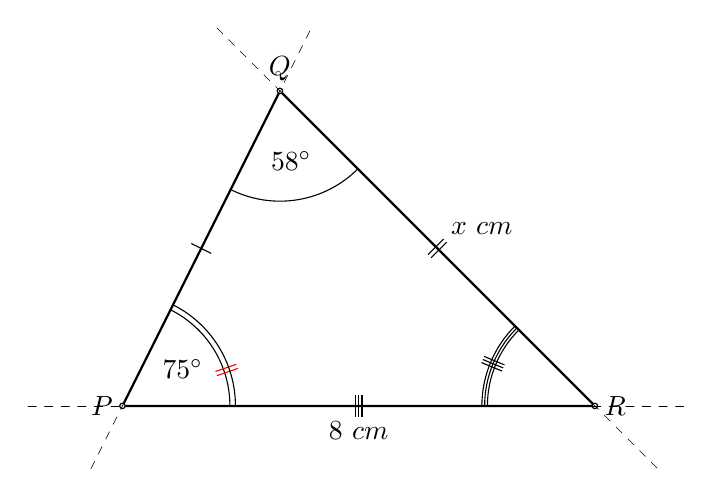
\begin{tikzpicture}
  %\draw[lightgray] (-1,-2) grid (7,5);

  \coordinate[label=left:$P$] (P) at (0,0);
  \coordinate[label=above:$Q$] (Q) at (2,4);
  \coordinate[label=right:$R$] (R) at (6,0);

  \draw[thick] (P)--(Q)--(R)--cycle;

  % label segments
  \tkzLabelSegment[below=2pt](P,R){$8\ cm$}
  \tkzLabelSegment[above right=2pt](Q,R){$x\ cm$}

  %mark angles
  \tkzMarkAngle[mark=||, arc=ll, mkcolor=red, mkpos=0.3, size=1.4](R,P,Q)
  \tkzMarkAngle[mark=none, size=1.4](P,Q,R)
  \tkzMarkAngle[mark=|||, arc=lll, size=1.4](Q,R,P)

  \tkzMarkSegment[mark=|](P,Q)
  \tkzMarkSegment[mark=||](Q,R)
  \tkzMarkSegment[mark=|||](P,R)

  \tkzLabelAngle[pos=0.9](R,P,Q){$75\degree$}
  \tkzLabelAngle[pos=0.9](P,Q,R){$58\degree$}

  \tkzDrawPoints(P,Q,R)
  \tkzDrawLines[dashed](P,Q Q,R P,R)

  %\coordinate[label=right: Diagram not drawn to scale] (G) at (5,-1.5);
\end{tikzpicture}  
\end{document}